\section{Introduction}

\begin{frame}[fragile,t]
    \begin{center}
        \begin{minted}{ocaml}
type 'a list =
| []
| (::) of 'a * 'a list

[] (* La liste vide *)
1 :: [] (* La liste contenant uniquement 1 *)
1 :: (2 :: []) (* La liste contenant 1, 2 *)
        \end{minted}

        \small Structures récursives

        \pause

        \begin{minted}{ocaml}
let rec sum (l : int list) : int =
    match l with
    | [] -> 0
    | x :: q -> x + sum q

sum [] (* 0 *)
sum (1 :: []) (* 1 *)
sum (1 :: (2 :: [])) (* 3 *)
        \end{minted}

        \small Fonctions récursives
    \end{center}
\end{frame}

\begin{frame}[fragile,t]
    \begin{minted}{ocaml}
let rec sum (l : int list) : int =
    match l with
    | [] -> 0
    | x :: q -> x + sum q

(* Stack overflow during evaluation (looping recursion?). *)
sum (List.init 1_000_000 (fun i -> i))
    \end{minted}
\end{frame}

\begin{frame}[fragile,t]
    \begin{minted}{ocaml}
let rec sum (l : int list) : int =
    match l with
    | [] -> 0
    | x :: q -> x + sum q
    \end{minted}

    \vspace{0.5cm}

    \begin{minted}{ocaml}
let sum (l : int list) : int =
    let res = ref 0 in
    let l_ref = ref l in
    while !l_ref <> [] do
        res := !res + List.hd !l_ref;
        l_ref := List.tl !l_ref
    done;
    !res

(* 499999500000 *)
sum (List.init 1_000_000 (fun i -> i))
    \end{minted}
\end{frame}

\begin{frame}
    \begin{center}
        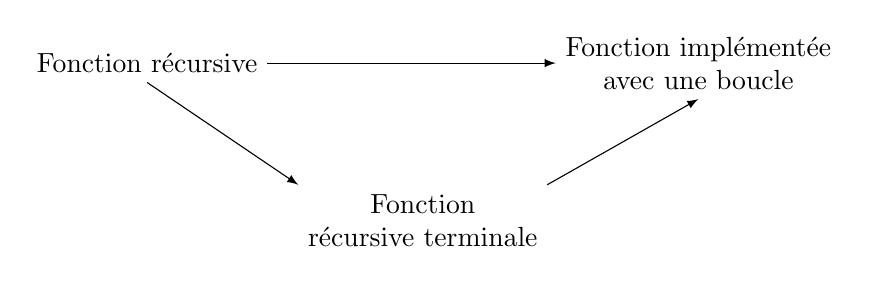
\begin{tikzpicture}
            \node (rec) at (-3.5, 0) {Fonction récursive};

            \node[align=center] (loop) at (3.5, 0) {Fonction implémentée \\ avec une boucle};

            \only<1>{
                \draw[-latex] (rec.east) to (loop.west);
            }

            \uncover<2->{
                \node[align=center] (terminal) at (0, -2) {Fonction \\ récursive terminale};

                \draw[-latex] (rec.south) to (terminal.north west);
                \draw[-latex] (terminal.north east) to (loop.south);
            }
        \end{tikzpicture}
    \end{center}
\end{frame}